\documentclass[a4paper,12pt]{scrartcl}


% deutsche Silbentrennung
\usepackage[english]{babel}
\let\latinencoding\relax
% eigene, zusätzliche Silbentrennung
\usepackage{hyphsubst} %Manuelle Sil\-ben\-tren\-nung
\usepackage[utf8]{inputenc}
\usepackage{amsmath}
\usepackage{amsfonts}
\usepackage{amssymb}
\usepackage{verbatim} 
\usepackage{hyperref}
 
  
% Seitenränder
\usepackage{geometry}
\geometry{a4paper, top= 25mm, bottom=20mm, left = 25mm, right = 25mm, footskip= 1cm}
\setlength\parindent{0pt}

\usepackage{graphicx}
%\includegraphics[width=0.5\textwidth]{images/img1} oder scale=1

% Zeilenabstand (Unterscheidet sich evtl von den Standard 1.5)
\usepackage{setspace}
\linespread{1.5}

\usepackage{fontspec}
%\setmainfont{Times New Roman}
\usepackage{booktabs}
\usepackage{multirow}
\usepackage{wrapfig}
%\usepackage{caption}

\usepackage{cancel}
\usepackage{csquotes}

\usepackage{colortbl}
\usepackage{xcolor}
%\usepackage{hyperref}
%\usepackage[all]{hypcap}
\usepackage{float}

\usepackage{pdfpages}
\usepackage[headsepline]{scrpage2}
\pagestyle{scrheadings}
\clearscrheadfoot

\ofoot{\pagemark}
\ohead{\normalfont \headmark}

%bibliography
\usepackage[natbib,style=alphabetic,minnames=2,maxnames=2,uniquelist=false,backend=biber]{biblatex}
\bibliography{bibliography}
\setlength{\bibitemsep}{1.5em}  

\automark{section}
\newcommand{\gr}{\grqq{}}
\newcommand{\gl}{\glqq}
\newcommand{\vs}{\vspace{3pt}}
\newcommand{\red}{{ \color{red} Quelle}} 
\newcommand{\LL}{\ensuremath{\mathcal{L}}}

\newcommand{\N}{\mathbb{N}}
\newcommand{\Z}{\mathbb{Z}}
\newcommand{\Q}{\mathbb{Q}}
\newcommand{\R}{\mathbb{R}}
%\newcommand{\C}{\mathbb{C}}
\newcommand{\F}{\mathbb{F}}

\renewcaptionname{english}{\figurename}{\small{Fig.}}
\renewcaptionname{english}{\tablename}{\small{Tab.}}
\newcommand{\norm}[1]{\left\| #1 \right\|}

\begin{document}
	
	
	\begin{singlespace}
		\begin{titlepage}
			\begin{center}
				
				
\includegraphics[scale=0.6]{wwu}
				
				\large{\textbf{\textsf{Faculty of Mathematics and Computer Science}}\\ 
					Summer Semester 2019} \\
				\vspace{20mm}
				\rule{.8\linewidth}{1pt}\\
				\vspace{3mm}
				\LARGE\textbf{\textsf{Behavioral Context Recognition In-The-Wild from Mobile Sensors}}\\
				%\rule{.2\linewidth}{.5pt}\\
				\rule{.8\linewidth}{1pt}\\
				
				\vfill
			\end{center}
			\begin{flushright}
				\flushright
				
				\begin{large}
					\singlespacing 		
					\begin{tabular}{rl}
						
						Authors: & Daniel Beckmann \\ & Joschka Strüber \\& Tony Prange \\& Thomas Poschadel \\
						\midrule
						Lecturers: & Prof. Xiaoyu Jiang \\
						& Sören Klemm \\
						Class:& Pattern Recognition \\ & and Machine Learning \\
						Submission deadline: & 13.09.2019
						
					\end{tabular}
				\end{large}	
			\end{flushright}
			
			\flushleft
		\end{titlepage}
		
		\newpage  \tableofcontents \thispagestyle{empty} \vspace{15mm}
		
		
	\end{singlespace}

\newpage
\setcounter{page}{1}

\section*{Abstract}

\todo{hier was schreiben}

\section{Introduction}
A large amount of data is available through the networking of our digital devices, which shape our everyday lives. The use of such data and the associated information is a core element of today's digital society. Programs that use such data to generate as much information as possible play an important role at assisting us and improving our daily lives. Those programs are used in great variety of real world contexts, not only at the level of targeted advertising, but also in improving our medical care and our behaviors. For example, many people are already optimizing their personal lifestyle with the assistance of digital devices like smartphones and fitness trackers. Another application lies in the establishment of a healthy sleep rhythm by the recognition of sleep phases. 

In the context of health care, this technology is of particular interest because on the one hand it can be used in a preventive manner. For example, people can be informed about their personal habits and sensitized to their personal risks which arise with their specific lifestyle in order to lead them to a healthier lifestyle, which in turn can be supported by technology again. On the other hand there is the medical perspective, where it is possible to check how healthy a person lives in order to combat diseases more effectively. In conclusion, deriving activities from various sensor data is important for many companies or health organizations, but also for the end user.

The present report was written during a practical course, led by Prof. Dr. Xiaoyi Jiang and Sören Klemm, with the topic \gl Behavioral context recognition in-the-wild from mobile sensors\gr{} accompanying the lecture Pattern Recognition. The aim of the project was to perform multi-label classification on the basis of the ExtraSensory data set. Essentially, collected sensor data should be assigned to activities, in an additional task the users should be recognized by their data. 

The particular challenge of the project was that firstly the methodology was not specified and secondly multi-label classification was to be carried out with a dataset containing many missing labels. 

\subsection{Introduction of the ExtraSensory Dataset}

The ExtraSensory dataset was collected in 2015 and 2016 by Yonatan Vaizman and Katherine Ellis under the supervision of Professor Gert Lanckriet. It is based on sensor data from smartphones and smartwatches produced by 60 participants in intervals of one minute. In contrast to many other datasets, the data was generated by normal everyday devices using multiple sensors at the same time. Furthermore, the participants behavior was not scripted like in many other case studies and they were allowed to behave in an natural way. The sensors included an accelerometer, gyroscope, location and audio sensor. Almost every participant used practically every sensor in the activity recordings. Additionally some participants used smart watches or fitness tracker which provided the additional watch accelerometer.

The users themselves assigned most of their data points to the respective activities. In the course of this they had the option to use predefined labels or create their own. The label represented various information about the location, the context and the activity of a user. Some examples are 'in class', 'singing', 'stairs (going up)', 'stairs (going down)', 'with friends' or 'talking'. In a preprocessing step these label were reduced to a set of 51 labels by combining similar labels. 

The final results contained 377,346 data points, which were described with one or more of the 51 final labels. 

\begin{figure}[H]
	\begin{center}
		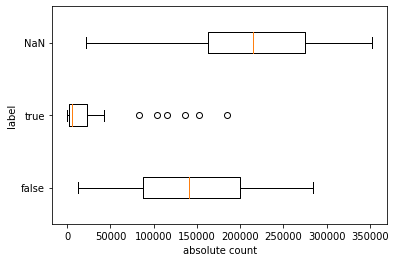
\includegraphics[scale=.8]{images/boxplot_label.png}
		\caption{A box-plot showing the distribution of the absolute count of a given value (false, true or NaN) over the different labels. The yellow line represents the median, the rectangle the 25\% percentile, the line the 75\% percentile and the dotes are outliers.}
		\label{abb:boxplot_label}
	\end{center}		
\end{figure}

\newpage
This means that for each data point a label vector of length 51 exists. Each entry can contain the values 'true', 'false' or 'NaN', where 'NaN' represents missing information on this label.

Figure \ref{abb:boxplot_label} visualizes the distribution of these values for each label as a box-plot diagram. Looking at the median for 'NaN', it can be seen that for most labels the majority of data points do not contain a value - which increases the difficulty of classification. This means that for many labels there exists a large number of data points in the ExtraSensory data set that do not contain any information regarding the label.

Furthermore, it can be seen that the median of labels with the value 'true' is just 5,153 meaning that in the median only 5,153 samples exist for a specific activity. Overall only very few labels at all are labeled as 'true' for more than 10\% of the data points, consequently there are many label classes consisting of very few representatives. 

\begin{figure}[h]
	\begin{center}
		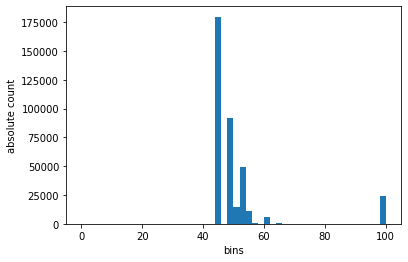
\includegraphics[scale=.8]{images/hist.png}
		\caption{Histogram of absolute counts of percentage of NaN values for each data point. The data is distributed into 50 bins. Each bin has the size of 2 \% of the labels.}
		\label{abb:histogramm_data}
	\end{center}		
\end{figure}

Finally, it can be seen that in all data points at least 44\% of the 51 labels are not evaluated. Thus, there are no data points that make statements about all labels at the same time, the data therefore is sparse in a variety of ways.

\subsection{State of the Art}

\section{Applied Theory}

\subsection{Random Forests}\label{subsec:random_forests}

A random forest is a classification method in which an ensemble of decision trees is created which are not correlated if possible. The underlying strategy, as with any ensemble classifier, is to create a stronger learner from weak learners. This is why the uncorrelatedness of the individual decision trees plays an important role, because the addition of a correlating tree hardly improves classification results in general. In the context of random forests, procedures exist to ensure low levels of correlations. One of these methods is found in feature subsampling where only a smaller subset of features is randomly chosen as training data in every iteration of decision tree creation. This method helps to prevent overfitting, because not every tree in the forest was trained on the same dataset. The evaluation of the ensemble usually takes place through some sort of a voting mechanism. \cite{Jiang}



\subsection{Gradient Boosting}\label{subsec:grad_boost}


The following section is based on \cite{Chen16} and \cite{Murphy}. Gradient boosting is about iteratively generating a set of gradient trees that solve a given classification problem as effectively as possible.

Gradient trees are essentially decision trees, except that each leaf of the tree has a value whose weight is assigned to $w_i$. Consequently, a gradient tree with $T$ leaves and corresponding weights $(w_1, ... ,w_T)$ can be understood as a function $f: \R^m \to \R$ . Each data point $x \in \R^m$ is assigned the weight of the leaf corresponding to $x$ by $f$ via $f(x) = w_{q(x)}$. The function $q: \R^m \to T$ assigns a sample $x$ to the index number of the leaf belonging to $x$. Furthermore $I_j := \{ i \mid q^{-1}(j)=x_i \}$ contains the indices of those samples which refer to the leaf number $j$. The set of all gradient trees is called $\mathcal{F}$.

A tree ensemble model $\{f_1, ... ,f_K \mid f_i \in \mathcal{F}\}$ consisting of $K$ gradient trees is not evaluated by voting, as known from decision trees, but by adding the function values of the sample $x$ of the single gradient trees in the ensemble function $\Phi = \sum f_k$. The predicted outcome $\hat{y}$ of a sample $x$ results from this:
$$\hat{y} = \Phi(x) = \sum_{k=1}^{K} f_k(x)$$
Given a sample set $X= \{x_1, ..., x_n\} \subset \R^{m} $ of $n$ samples each with $m$ features and the corresponding ground truths $\{y_1, ... ,y_n\}$, the resulting regularization function is found in:	
$$\mathcal{L} = \sum_{i=1}^{n} l(y_i, \Phi(x)) + \sum_{k=1}^{K}\Omega(f_k) \text{,  where } \Omega(f_k) = \gamma T + \frac{1}{2}\lambda \norm{w}_2^2$$
$l$ is the loss-function, a convex and several times differentiable function. $\Omega$ is a penalizing term in this context and monitors the structure of the tree within $\LL$. The choice of $\gamma$ influences the number of permissible leaves and $\lambda$ influences their weights. Thus $\Omega$ is a preventive measure against overfitting. Consequently, the model created with $\LL$ prefers gradient trees of simple shape.

\begin{figure}[H]
	\begin{center}
		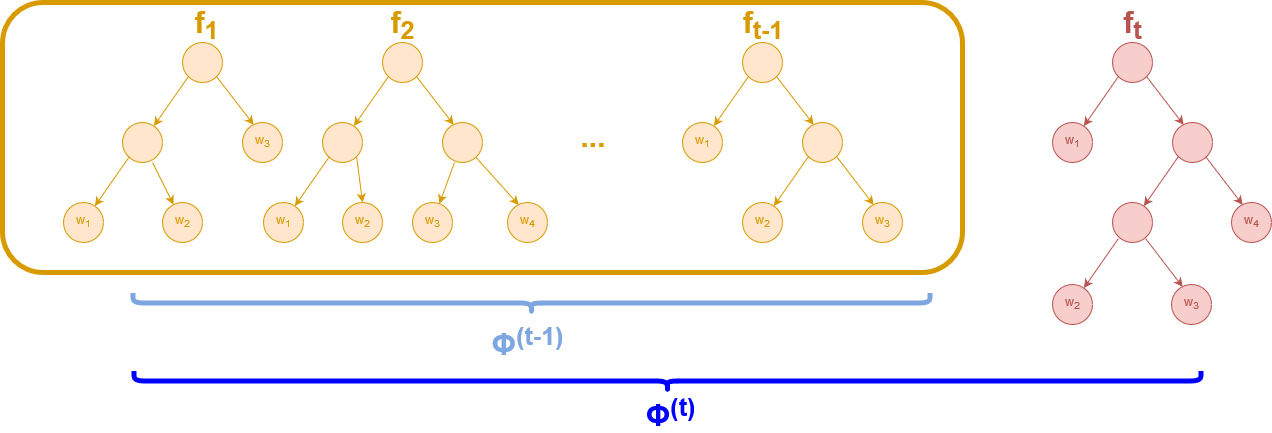
\includegraphics[width=\textwidth]{images/gradient_boosting.png}
		\caption{Visualisation of the $t$-th iteration step: For a fixed tree $f_t$ its weights $w_i$ have to be optimized with respect to the already existing set of trees.}
		\label{abb:gradient_boosting}
	\end{center}		
\end{figure}
The actual gradient tree boosting takes place by iteratively adding new trees to the ensemble. In the $t$-th iteration step, the ensemble consists of the gradient trees $\{f_1, ... , f_{t-1}\}$ created in the previous steps. The goal is to select the new gradient tree $f_t$ so that it improves the current model the most. This is the case if and only if 
\begin{equation}
\LL^{(t)} = \sum_{i=1}^{n} l(y_i, \Phi(x_i)) + \sum_{k=1}^{K}\Omega(f_k)
\label{eq:LL1}
\end{equation}
is minimized.

Since the $\Omega(f_k)$ for the trees $f_1, ... f_{t-1}$ are already fixed, they play no role in the consideration. Further established are the first $t-1$ terms of the sum $\Phi(x_i) = f_1(x_i) + ... + f_{t-1}(x_i) + f_t(x_i)$. This sum is constant and is aggregated in the expression $\hat{y}^{t-1}$, because it represents the predicted outcome after the $t-1$-th iteration step of the ensemble.

With this (\ref{eq:LL1}) can also be formulated as:
\begin{equation}
\LL^{(t)} = \sum_{i=1}^{n} l(y_i, \hat{y}^{(t-1)} + f_k(x_i)) + \Omega(f_t)
\label{eq:LL2}
\end{equation}

To separate the dependence of $l$ and $f_t$, the 1D-taylor series expansion is executed at the location $(y_i,\hat{y}^{(t-1)})$ on the function $l$ and only in the second coordinate. Although $l$ is a 2D function, changes in the context of $\LL$ only take place in one coordinate, which is why it is allowed to interpret it as a 1D function - like $l(y_i,x) = l_{y_i}(x)$. It results:
\begin{equation}
\label{eq:taylor}
l_{y_i}(\hat{y}^{(t-1)} + f_k(x_i)) = l_{y_i}(\hat{y}^{(t-1)}) + l_{y_i}^{'}(\hat{y}^{(t-1)}) \cdot f_k(x_i)
+ \newline \frac{1}{2} l_{y_i}^{''}(\hat{y}^{(t-1)}) \cdot f_k(x_i)^2 + R_\text{taylor}
\end{equation}

For readability's sake we write $g_i = l_{y_i}^{'}(\hat{y}^{(t-1))}) ) = \frac{\partial l}{\partial \hat{y}^{(t-1)}}(y_i,\hat{y}^{(t-1)})$ and $h_i = l_{y_i}^{''}(\hat{y}^{(t-1)}) ) = \frac{\partial l}{\partial^2 \hat{y}^{(t-1)}}(y_i,\hat{y}^{(t-1)})$. The $g_i$ and $h_i$ are constants, because both $y_i$ and $\hat{y}^{(t-1))}$ are known in the current iteration step. If we apply the findings from equation (\ref{eq:taylor}) to $\LL^{(t)}$, we get the result:
\begin{equation} \label{eq:shortL}
\LL^{(t)} \approx \sum_{i=1}^{n} (l(y_i,\hat{y}^{(t-1)}) + g_if_t(x_i) + \frac{1}{2} h_i f_t(x_i)^2) + \Omega(f_t)
\end{equation}

Since the constant terms $l(y_i,\hat{y}^{(t-1)})$ do not depend on $f_t$, they can be ignored in the optimization problem and the result is the simplified objective:
\begin{equation} \label{eq:LLeinfach}
\tilde{\LL}^{(t)} = \sum_{i=1}^{n}( g_if_t(x_i) + \frac{1}{2} h_i f_t(x_i)^2) + \Omega(f_t)
\end{equation}

This term can now be simplified by writing out $\Omega(f_t) = \gamma T + \frac{1}{2}\lambda \sum_{j=1}^{T} w_j^2$. For a given tree structure $q$ we get the different $I_j$ which can be used to change the summation order. For this, $f_t(x_i)$ is expressed as the corresponding weight $w_j$ of the new tree $f_t$. The rearrangement is done by sorting by the appearing $w_j$. Applied to (\ref{eq:LLeinfach}) this results in:
\begin{equation} \label{eq:LL_umsortiert}
\tilde{\LL}^{(t)} = \sum_{j=1}^T\left( (\sum_{i \in I_j} g_i) w_j + \frac{1}{2} (\sum_{i \in I_j} h_i + \lambda)w_j^2 \right) + \gamma T
\end{equation}

It should be noted that for this rearrangement and a concrete evaluation of the term of the above equation a \textit{fixed} tree structure $q$ must be provided. This means that the tree must already be fixed except for the weights of its leaves.

To find the optimized weights $w^*_j$ for this fixed structure of $f_t$, derive $\tilde{\LL}^{(t)}$ from equation (\ref{eq:LL_umsortiert}) in the direction of the corresponding $w_j$ and it yields:
\begin{equation} \label{eq:LL_ableitung}
\frac{\partial \tilde{\LL}^{(t)}}{\partial w_j} = \sum_{i \in I_j} g_i + (\sum_{i \in I_j} h_i + \lambda)w_j
\end{equation}

By setting this equation to $0$ and solving it for $w_j$, the optimal $w^*_j$ is gained, which minimize $\tilde{\LL}^{(t)}$:
\begin{equation} \label{eq:opt_w}
w_j^* = - \frac{\sum_{i \in I_j} g_i}{\sum_{i \in I_j} h_i + \lambda}
\end{equation}

Using this optimal $w_j^*$ in (\ref{eq:LL_umsortiert}) results in the optimal value of $\tilde{\LL}^{(t)}$ for the tree structure $q$:
\begin{equation} \label{eq:entropy}
\tilde{\LL}^{(t)} (q) = - \frac{1}{2} \sum_{j=1}^{T} \frac{(\sum_{i \in I_j} g_i)^2}{\sum_{i \in I_j} h_i + \lambda} + \gamma T
\end{equation}

So it is possible to calculate for a given tree structure $q$ the most helpful weights of the new tree $f_t$ for the ensemble using (\ref{eq:opt_w}). Furthermore, such an (optimized) tree structure $q$ can be evaluated with (\ref{eq:entropy}), this rating is comparable to the entropy of decision trees. 

In reality one would have to work through all possible tree structures, including the different feature-splits, the optimized $w^*_j$ and $\tilde{\LL}^{(t)} (q)$ and compare. Because this is hardly realizable, the new tree $f_t$ is constructed in the iteration step $t$ by a greedy algorithm. In this process, branches are added iteratively to the tree by splitting a leaf. Let $I_l, I_r$ be the sets of the index numbers assigned to the left or right leaf and $I = I_l \dot\cup I_r$ the index set of the former leaf. The resulting improvement of this split results after (\ref{eq:entropy}):
\begin{equation} \label{eq:LRsplit}
	\begin{split}
		\tilde{\LL}_\text{split} &= \tilde{\LL}^{(t)} (q_\text{alt})-\tilde{\LL}^{(t)} (q_\text{neu})\\
		&= \left( - \frac{1}{2} \sum_{j=1}^{T} \frac{(\sum\limits_{i \in I_{j, \text{alt}}} g_i)^2}{\sum\limits_{i \in I_{j, \text{neu}}} h_i + \lambda} + \gamma T \right)- \left( - \frac{1}{2} \sum_{j=1}^{T+1} \frac{(\sum\limits_{i \in I_{j, \text{neu}}} g_i)^2}{\sum\limits_{i \in I_{j, \text{neu}}} h_i + \lambda} + \gamma (T+1) \right)\\	
		&= \frac{1}{2} \left( \frac{(\sum_{i \in I_l} g_i)^2}{\sum_{i \in I_l} h_i + \lambda} + \frac{(\sum_{i \in I_r} g_i)^2}{\sum_{i \in I_r} h_i + \lambda} - \frac{(\sum_{i \in I} g_i)^2}{\sum_{i \in I} h_i + \lambda} \right) - \gamma 
	\end{split}
\end{equation}

The second equality follows from the fact that the index sets $I_j$ do not differ except for the split leaf, i.e. the index sets $I, I_l$ and $I_r$, and thus cancel each other out.




\subsection{XGBoost}

According to the theory of gradient boosting, every implementation of gradient boosting has to deal with the problem that all possible splits have to be sensibly reduced and evaluated with a useful systematic  efficiently.

Compared to other tree boosting systems like scikit-learn, XGBoost supports the exact greedy algorithm, approximate global and local algorithms of split-finding which means that we had the option using all three, is a fitting situation should arise. Furthermore XGBoost includes several additional measures against overfitting and efficiency considerations like \textcolor{red}{out-of-core, sparsity aware and parallel}.  All this led to our decision to use XGBoost.

\subsubsection{XGBoost: Spardity-Awareness}

Especially the sparsity-awareness of XGBoost played a huge role in our choice, since the underlying dataset itself is consisting of mostly missing data - as mentioned before.

To deal with missing entries, XGBoost assigns a default branch to each tree node. This default branch is used by samples that do not have an assigned value at the corresponding location. The default branch is learned by a dedicated algorithm during the process itself. A score is assigned to each possible branch, based on the samples that possess a corresponding feature value and pass through the branch.

This is an obvious improvement over the procedure of simply setting all missing values to a certain, fixed value in advance.

\subsubsection{XGBoost: greedy and approximate algorithm}
The greedy algorithm iterates over all possible splits of a current leaves, evaluating equation (\ref{eq:LRsplit}) and picking the split with the best result. As mentioned above this process is not very efficient. The solution given by XGBoost consists in two different approximate algorithms: the local and the global one.

\newcommand{\rnk}{\operatorname{rank}}
At the center of both algorithms resides the idea that not all feature-values should be tested as possible feature-splits. Instead, the algorithms look for a set of representatives on the basis of which the continuous features are divided into buckets. This is achieved as follows: For the feature vector $x_i$, $x_i,k$ denotes the value of the $k$-th feature, and $h_i$ and $g_i$ indicate the values corresponding to $x_i$ introduced in the equation (\ref{eq:shortL}).
A ranking-function $\rnk_k : \R\to \R_{\geq 0}$ can be established:

\begin{equation} \label{eq:ranking}
	\rnk_k(\zeta) = \frac{\sum\limits_{i: x_{i,k} < \zeta} h_i}{\sum\limits_{i=1}^n h_i}
\end{equation}

where $n$ represents the number of total samples. $\rnk_k(\zeta)$ indicates the weight of samples that have a feature-value smaller than $\zeta$. In this context, $h_i$ is a proper weight, since equation $\ref{eq:shortL}$ can be transformed into weighted square loss with weights $h_i$ by putting $h_i$ outside the brackeds and completing the square with $\frac{g_i}{h_i}$.

For a fixed $\epsilon$, the representatives of the $k$-th feature $\{r_{k,1}, ... .r_{k,m}\}$, with $r_{k,1} = \min x_{i,k}$ and $r_{k,1} = \max x_{i,k}$, are found using the following property:

\begin{equation}
	\mid \rnk_k(r_{k,i}) - \rnk_k(r_{k,i+1}) \mid < \epsilon
\end{equation}

This means that the representatives $r_{i,k}$ decompose the feature-values $x_{i,k}$ of the $k$-th feature in such a way that there is approximately the same weight (a weight smaller than $\epsilon$) between two adjacent representatives.

A good choice of $\epsilon$ is decisive for the resulting performance, since it controls the finding of representatives. In the further course, the resulting intervals between representatives are used, which can mean a big leap in efficiency regarding the greedy method.

The difference between the global and local variant of the algorithm resides in the fact that in the global version the candidates are created only once at the beginning of the construction of the tree, in the local version these are determined again after each iteration under consideration of the feature choices made.

\subsubsection{XGBoost: Avoiding overfitting}
Besides the term $\Omega$ XGBoost uses two main strategies to avoid overfitting: shrinkage and feature subsampling. With shrinkage, each tree, or more precisely its weights, is given a factor according, which is taken into account when the ensemble is evaluated. Essentially there is the possibility to shrink all previous trees, i.e. to add a factor to $\sum\limits_{k=1}^n f_k(x)$, or to add a factor to the new tree $f_t$. Both versions have the same effect by either shrinking the existing forest or increasing the size of the new tree. Similar to the learning rate in other contexts, shrinkage allows to vary the effect of future trees on the ensemble. Feature subsampling is the same strategy known from random forests.



\subsection{Naive Bayes}
The goal of every classification task is to estimate the probability for a class $y$ to be present when given a set of features. This probability is given by
\begin{equation}
	P(y|(x_1,\dots,x_n)).
\end{equation}
Under the \glqq naive\grqq assumption (this gave the name of this classification method) that all features $(x_1,\dots,x_n)$ are pair-wise conditionally independent, the probability for a class $y$ can be rewritten by applying Bayes' Theorem:
\begin{equation}
	P(y|(x_1,\dots,x_n)) = \frac{P(y)\Pi_{i=1}^{n} P(x_i|y)}{P(x_1,\dots,x_n)}.
\end{equation}
Since $P(y)$ can easily be estimated by calculating the relative appearance ratio in the data set and $P(x_1,\dots,x_n)$ is independent of class $y$, the only task left is to estimate the distribution $P(x_i|y)$ for all features. One popular approach is to assume that the likelihood of feature is Gaussian, that is
\begin{equation}
	P(x_i|y) = \frac{1}{\sqrt{2\pi \sigma_y^2}}\exp\left(-\frac{(x_i-\mu_y)^2}{2\sigma_y^2}\right).
\end{equation}
The mean $\mu_y$ and variance $\sigma_y^2$ is then calculated using maximum likelihood. (For details on how to do this, please refer to the Pattern Recognition course by Prof. Jiang)

\subsection{Logistic Regression}
Logistic Regression is another method for classification which utilizes the logistic sigmoid function. In this context, a two-class classification problem is assumed for simplicity's sake. The function is obtained by using the property of $b = \exp(\ln(b))$ on 

\begin{equation}
	p(C_1|x)  = \frac{p(x|C_1)P(C_1)}{p(x|C_1)P(C_1)+p(x|C_2)P(C_2)}
\end{equation}

where $x$ is an element from the $M$-dimensional feature space $X$. Substitution returns the sigmoid function 

\begin{equation} \label{eq:sigmoid}
\sigma(a) = \frac{1}{1 + \exp(-a)} \text{, where } a = \ln\frac{p(x|C_1)P(C_1)}{p(x|C_2)P(C_2)}
\end{equation}
which also represents the probability $p(C_1|x)$. 

The logistic regression model is defined as shown in (\ref{eq:logreg_model}) and describes the probability of a feature to be in class $C_1$:
\begin{equation} \label{eq:logreg_model}
p(C_1|x) = y(x) = \sigma(w^\text{T}x)
\end{equation}
Here $w$ is a set of parameters with the same dimension $M$ as the feature space $X$, that needs to be optimized to best fit the data, and $\sigma$ is the logistic sigmoid function (\ref{eq:sigmoid}). The probability of the feature $x \in X$ to be from class $C_2$ is then trivially given by $p(C_2|x) = 1 - p(C_1|x)$. To determine the $M$ parameters of the logistic regression model, the derivative of the logistic sigmoid function can be used, which is conveniently expressed by the sigmoid function itself:
\begin{equation} \label{eq:sigmoid_derived}
\frac{\partial \sigma}{\partial a} \overset{\text{chain}}{\underset{\text{rule}}{=}} \frac{\exp(-a)}{(1+\exp(-a))^2} = \frac{1}{1+\exp(-a)} \cdot \frac{\exp(-a)}{1+\exp(-a)}= \sigma \cdot(1-\sigma)
\end{equation}
For a given data set $X = \{(x_1,t_1), .. , (x_N,t_N)\}$, where $t_n = \mathbbm{1}_{C_1}(x_n) \in \{0,1\}$ the likelihood function can be written as
\begin{equation} \label{eq:likelihood_function}
p(t|w)=\prod_{n=1}^{N}y_n^{t_n} (1-y_n)^{1-t_n}
\end{equation}
where $t=(t_1, \dots, t_N)^\text{T}$ and $y_n = \sigma(w^\text{T}x_n)$. 
The negative logarithm applied to (\ref{eq:likelihood_function}) results in an error function, which is utilized to find the best parameter for $w$:
\begin{equation} \label{eq:likelihood_function}
E(w)=-\ln p(t|w) = - \sum_{n=1}^{N}t_n \ln y_n + (1-t_n) \ln (1-y_n)
\end{equation}
where $y_n=\sigma(w^\text{T}x_n)$. Using equation (\ref{eq:sigmoid_derived}) and taking the gradient with respect to $w$ by using chain and sum rule of derivation we obtain:
\begin{equation} \label{eq:lin_reg_gradient}
\begin{split}
\nabla E(w) &= - \sum_{n=1}^{N} \left( t_n \frac{1}{y_n} y_n(1-y_n)x_n + (1-t_n)\frac{1}{1-y_n}(-y_n)(1-y_n)x_n \right)\\ &=\sum_{n=1}^{N} (y_n-t_n)x_n
\end{split}
\end{equation}
This function can be used to fit the best parameters.
The advantage of the logistic regression is that it uses $M$ parameters to fit to a $M$-dimensional feature space and grows linear with the dimension of the feature space, in contrast to, e.g. fitted Gaussian class conditional densities using maximum likelihood which grows exponentially with the dimension $M$. It should be noted, that this whole procedure is also applicable if a nonlinear transformation $\Phi$ to another feature space (of higher dimension) is applied to the data set $X$. In this case, all $x_n$ only have to be replaced by $\Phi_n = \Phi(x_n)$. \cite{Bishop}

\subsection{Support Vector Machine}

\subsection{correlation stuff}

\subsection{Bayesian Optimization}\label{subsec:bayes_opt}
In general, the goal of any optimization is to find the global (or a local) minimum/maximum of some function $f(x)$ on some input set $\mathcal{X}$. In our case, this function is identified with our classifier, whereas $x$ can be interpreted as a point in the corresponding hyperparameter space, and $f(x)$ is the measured accuracy of our classifier for this particular set of hyperparameters. Since this function cannot be expressed with an explicit formula, analytical methods for calculating extrema cannot be applied. Numerical methods which require a lot of iteration before convergence are also problematic, since calculating $f(x)$ is computationally expensive. \par
Bayesian Optimization tries to find the maximum of $f$ by constructing a probabilistic model of this function, which is updated and enhanced in every iteration. Basis for this model is a Gaussian Process. Stochastic processes in general are defined as a (infinite) set of random variables which can be indexed (by time or some underlying space; in our case, this is the hyperparameter space). A stochastic process is now called Gaussian, if any finite collection of those random variables has a multivariate normal distribution, i.e. every finite linear combination of random variables from this process is normally distributed. \par
Given a set of observations $\{x_i,y_i\}$ which are found by testing the classifier with some sets $\{x_i\}$ of hyperparameters, the probalistic model together with these observations induce a so-called \emph{acquisition function} (also known as \emph{utility function}) $a: \mathcal{X} \rightarrow \mathbb{R}^+$ , which then is used to calculate the next point $x_{\text{next}} \in \mathcal{X}$ which will be evaluated. \cite{snoek2012practical}

\begin{figure}[H]
	\begin{center}
		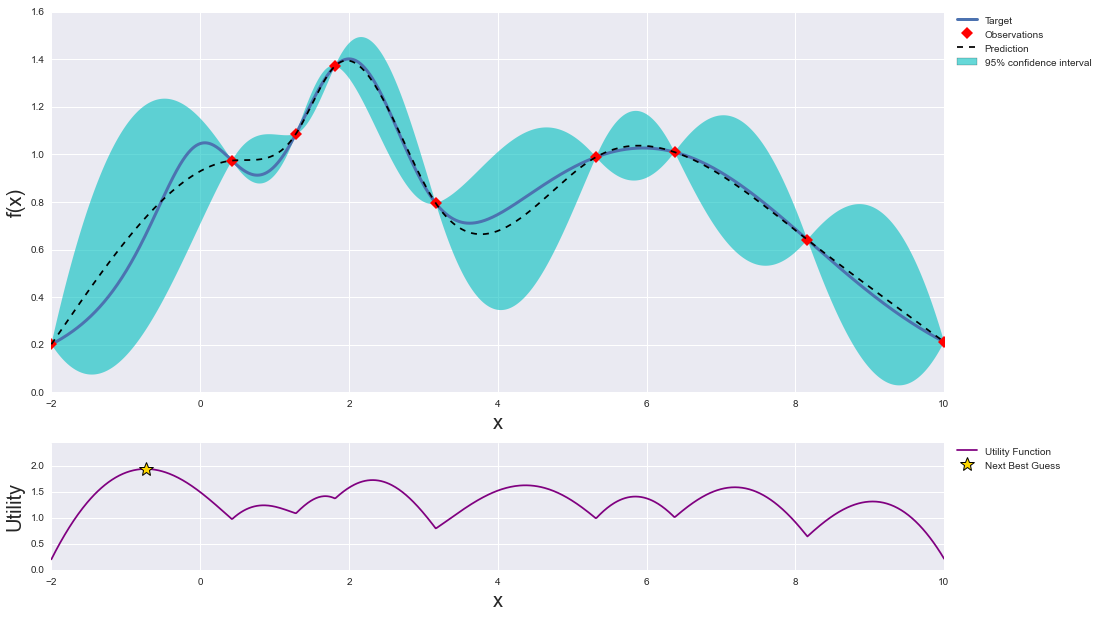
\includegraphics[width=\textwidth]{images/bayesian_optimization_example.png}
		\caption{Toy-example with one-dimensional $f(x)$. The target function also is displayed. Taken from the official Github implementation for Bayesian Optimization. Source: \href{https://github.com/fmfn/BayesianOptimization}{github.com/fmfn/BayesianOptimization}}
		\label{abb:bayes_opt_example}
	\end{center}		
\end{figure}
In our implementation, Bayesian Optimization is used in the One-vs-Rest-Classifier to optimize the hyperparameters of each individual internal classifier. 

\section{Handling Missing Labels}
One of the great challenges of the dataset is the large number of missing labels. For each of the 51 labels, at least 43\% of the samples lack an assignment (see figure \ref{abb:histogramm_data}). In order to maximize the amount of samples for each label, it would be advantageous to obtain all missing values and thus completing the label matrix. One simple approach is to fill in the missing labels with fixed values or using the mean or median of the other values known for this label. In the following, two more advanced approaches are presented that perform a general matrix completion.

\begin{subsection}{Soft-Impute}
	In order to fill a thin matrix $X$ with unknown values, it is assumed that a low-rank representation $Z$ of $X$ exists. Iterative algorithms now search for such a representation in the form of the following optimization problem:
	\begin{equation} \label{eq:low-rank-opt}
		\begin{split}
			\text{minimize } &\operatorname{rank}(Z) \\
			\text{subject to } &\sum_{(i,j)\:\in\: \Omega} (X_{ij} - Z_{ij})^2 \leq \delta
		\end{split}	
	\end{equation}
	Here $\Omega$ denotes the set of all indices for which $X$ contains values. The regularization parameter $\delta$ determines the maximum deviation of the generated matrix $Z$ from the original one by means of the sum-of-squares error. To calculate the values in $Z$, an SVD is performed and the new values for $Z$ are calculated with the help of this SVD and regard to the constraints to be optimized.\par
	The original optimization problem (\ref{eq:low-rank-opt}) is considered in Soft Impute in a slightly modified form. The rank of the matrix $Z$ is replaced by the nuclear norm, which is defined as the sum of the singular values of a matrix \cite{mazumder2010spectral}.
	\begin{equation} \label{eq:low-rank-soft-opt}
	\begin{split}
	\text{minimize } & \| Z \|_* \\
	\text{subject to } &\sum_{(i,j)\:\in\: \Omega} (X_{ij} - Z_{ij})^2 \leq \delta
	\end{split}
	\end{equation}
	Since the algorithm is specifically designed to handle large matrices with up to millions of rows and columns, this method converges pretty quickly (around 2 - 5 minutes) on our label matrix, which only contains about 300000 rows with 51 entries each. 
\end{subsection}

\begin{subsection}{Iterative Impute}
	Another approach is to handle features as functions of other features. More precisely, if a feature (label in our context) has missing values, the known ones are interpreted as the output of a function, that takes all the other existing features from the corresponding sample as input. In other words, we interpret problem of missing values as a regression task based on the present labels. \par
	Iterative Impute now tries to estimate these functions in a round-robin fashion. Each round, one feature (e.g. label) with missing values is selected, for which an estimating function is then calculated. This is done by training a regressor with our selected feature as the target, and all the other features as input data. The missing values for our feature are then calculated by the trained regressor. This whole process for all features is then repeated for a given number of iterations. For every feature in each round a regressor needs to be trained. Naturally, this method does require substantially more time to converge than Soft Impute, up to one hour on our data set. \par
	
	For this algorithm, we used the experimental implementation provided by Scikit-Learn\footnote{\href{https://scikit-learn.org/stable/}{https://scikit-learn.org}}, which is based upon a work on imputation algorithms in R \cite{buuren2010mice}.
\end{subsection}

\begin{subsection}{Experimental Results}
	Since both algorithms are not specifically designed to fill in missing labels for classification problems - unlike algorithms such as matrix co-completion (\cite{Xu18}) - our expectations regarding an improvement in classification of activities were limited. Despite that, some of the labels seem to be naturally correlated, such as \emph{sleeping} and \emph{lying down}. Using this information to identify such a low-rank representation of our label matrix seemed somewhat promising. Actually, Soft Impute did find a representation of lower rank, around rank 45-47, depending on which portion of the data set was used to train. The following table shows the experimental results for both label imputing strategies. We used 5-fold cross validation with the same splits for every strategy, including no imputation. We used XGBoost as a classifier with hyperparameters found by Bayesian Optimization:
	\begin{table}[H]
		\begin{center}
		\caption{Balanced Accuracy on each split for different imputing strategies}
		\begin{tabular}{r||c|c|c|c|c|c}
			\toprule
			& 1st run &2nd run &3rd run& 4th run & 5th run & avg\\
			\midrule
			No imputation&0.6524&0.6452&0.6801&0.6751&0.6704&\textbf{0.6646}\\
			
			Soft imputation&0.6300&0.6445&0.6496&0.6291&0.6364&\textbf{0.6380}\\
			Iterative imputation&0.6317&0.6423&0.6601&0.6289&0.6426&\textbf{0.6411}\\
			\bottomrule
		\end{tabular}		
		\end{center}	
	\end{table}

	Our experiments show that imputing the label matrix with algorithms based on normal matrix completion do not improve the classification results. A reason for this could be that found correlations between labels may only exist when the label matrix is considered independently. A more sophisticated approach would be to search for correlations which are based on the feature matrix as well. \par
	We decided not to use a label imputation algorithm. Instead, each classifier is only given those samples from the dataset, for which its corresponding label is set.
\end{subsection}

\section{implementation}
-> Metric

\section{discussion}

\section{classification of users}




\newpage
\section{Literaturverzeichnis}
\printbibliography
\hangindent+30pt \hangafter=1
\textsc{Drüke-Noe, C.} 2014. \textit{Aufgabenkultur in Klassenarbeiten im Fach Mathematik – Empirische Untersuchungen in neunten und zehnten Klassen}. Wiesbaden:
Springer Spektrum.









\newpage
\ohead{\normalfont Declaration of Academic Integrity}
\addcontentsline{toc}{section}{Declaration of Academic Integrity} 
\vspace*{1cm}
\begin{center}
	\Large \textbf{Declaration of Academic Integrity}\\
	
	\large \textbf{Anti-Plagiarism Statement}
\end{center}

\normalsize
\vspace{25mm}
We hereby certify that we have written this work \grqq Behavioral Context Recognition In-The-Wild from Mobile Sensors\grqq{} independently, that we have not used any other sources and means than those indicated, and that the parts of the work taken from other works - including electronic media - have in any case been identified as borrowed, stating the source.\\
	
	
	
	


\begin{center}
	\rule{6cm}{.5pt} \hspace{3cm} \rule{6cm}{.5pt}
\end{center}
\vspace{1cm}
\begin{center}
	\rule{6cm}{.5pt} \hspace{3cm} \rule{6cm}{.5pt}
\end{center}

\vspace{3cm}
	\begin{center}
	\rule{6cm}{.5pt} \hspace{3cm} \rule{6cm}{0pt}
\end{center}	
\vspace{-5mm}
\hspace*{25mm} Ort, Datum	

\end{document}